\section{Virtualised Network Functions in \headershortacr{3G} Core Networks}\label{sec:cloud:virtualized_network_functions}
\newcommand{\blockingprobability}[0]{\ensuremath{p_B}\xspace}
\newcommand{\maxServers}[0]{\ensuremath{S_{\max}}\xspace}
In this section we apply the theoretical methods discussed in \refsec{sec:cloud:data_centers} and apply them to the real-world challenge of virtualised network functions.
We consider the exemplary use case of a virtualised \gls{GGSN}.
Here, network operators consider the virtualisation of previously physical middleboxes, in order to gain elasticity and reduce costs.

In contrast to the last section, we assume a loss model, as connection establishment requests are not queued in reality but expire if no capacity is available.
Thus, we consider the blocking probability instead of the mean waiting time as a metric.
As a second metric we consider the number of provisioned servers which need to kept powered on. 

This section is structured as follows:
In \refsec{sec:cloud:virtualized_network_functions:model} we first introduce a model for a traditional \gls{GGSN}.
Then, we extend it to be applicable for the study of a virtualised \gls{GGSN}.
In \refsec{sec:cloud:virtualized_network_functions:measurement_data} we describe the procedures used to obtain and process input parameters for use in our simulation study.
Finally, in \refsec{sec:cloud:virtualized_network_functions:performance_evaluation} we study possible gains by a virtualised \gls{GGSN} by considering the tradeoff between the required servers to be active simultaneously and the incurred blocking probability. 

\subsection{Models of \headershortacr{GGSN} Implementations}\label{sec:cloud:virtualized_network_functions:model}

In this section we provide a model for a traditional \gls{GGSN} and discuss a model for a virtual \gls{GGSN} using \gls{NFV}.
In \gls{NFV} \cite{Nfv2013} static network middleboxes are replaced by commodity hardware.
The tasks solved by the original middleboxes are then solved by dedicated software.

\subsubsection*{Traditional GGSN}\label{sec:cloud:virtualized_network_functions:model:traditional_ggsn}
First, we give a model for a \emph{traditional} \gls{GGSN}, i.e. a static network component.
While we consider the \gls{GGSN} to be one fixed entity, it can in reality consist of multiple servers.
However, due to the fact that the \gls{GGSN} is purchased from a vendor as a middlebox, idle servers can be neither deactivated nor reused for other purposes.

\begin{figure}
  \centering
  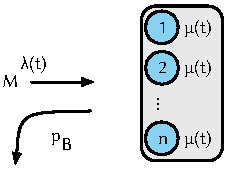
\includegraphics{cloud/virtualized_network_functions/model/figures/traditional_ggsn}
  \caption{Considered model of a traditional \headershortacr{GGSN}.}
  \label{sec:cloud:virtualized_network_functions:model:traditional_ggsn:model}
\end{figure}

We present an abstract queueing model for the traditional \gls{GGSN} in \reffig{sec:cloud:virtualized_network_functions:model:traditional_ggsn:model}.
New tunnels requests arrive according to a Poisson process with rate \(\lambda(t)\) at the \gls{GGSN}.
This server will support a maximum tunnel capacity of \(c\).
When this capacity is reached, blocking will occur and newly incoming tunnels requests are rejected.
Traditionally, \glspl{GGSN} can be expected to be overdimensioned in such a way that this rarely happens.
If the new tunnel is accepted, it will occupy one of the serving units of the server for the duration \(\mu(t)\) of the tunnel.
As stated earlier, we can not model the tunnel duration to be markovian, resulting in a  \(M/GI/c\) loss system.
In order to give quality of service guarantees the network operator is interested in the system's blocking probability \(\blockingprobability\), which we consider to be a key metric of our model.
Additionally, the previously described diurnal patterns can also be modelled by adjusting the arrival and serving process distributions for each time of day.
This alternatively also allows just to investigate the busy hour and thus the system's peak load.

\subsubsection*{\headershortacr{GGSN} using Network Function Virtualisation}\label{sec:cloud:virtualized_network_functions:model:virtual_ggsn}
Next, we introduce concepts from \gls{NFV}, i.e. the idea to replace middleboxes with commodity hardware as an extended model in \reffig{sec:cloud:virtualized_network_functions:model:virtual_ggsn:model}.
This allows us to realise benefits from cloud computing, as we are now able to scale out, instead of up.
The assumptions of the Markov arrival process \(\lambda(t)\) and the serving time distributions \(\mu(t)\) are carried over.
However, instead of one server processing every tunnel, this model assumes that there are up to \(s_{max}\) virtualised servers \(s_i\).
Each of these is less powerful than the traditional \gls{GGSN}, having a tunnel serving capacity of \(c_i \ll c\) and a total system capacity of \(c_{max} = s_{max} \times i\).

\begin{figure}
  \centering
  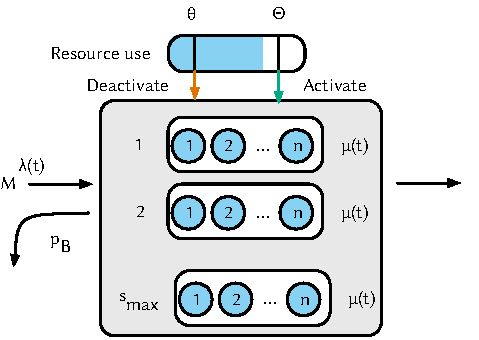
\includegraphics{cloud/virtualized_network_functions/model/figures/virtual_ggsn}
  \caption{Considered model of a virtualised \headershortacr{GGSN}.}
  \label{sec:cloud:virtualized_network_functions:model:virtual_ggsn:model}
\end{figure}

In its initial state, for efficiency, all but a small portion of the server instances are considered to be disabled.
Only, when a certain condition is reached, a new server instance is provisioned.
As a simple example, one instance could be kept in reserve for upcoming requests and an additional would be provisioned as soon as the reserve is used.
Similar rules should apply to the shut-down of servers and form a hysteresis with the boot condition.
For example it would be possible to keep at least one server in reserve but never more than two.

If these conditions are not carefully selected and are in tune with the expected boot time of an instance, additional blocking can occur.
Despite not having reached its maximum capacity, this system would still reject tunnel requests during the provisioning phase when no tunnel slots are available.
This could be remedied by a request queue.
However, this would introduce additional complexity to the system without providing real benefit, as mobile devices or applications will repeat their attempts and would timeout when the request is taking too long.

To place incoming tunnel state on one of the available servers a load balancer is required.
To ensure that the system in run time can scale down to its actual needs, the balancer should place tunnels on servers that are the fullest, keeping the reserve free.
It may even migrate tunnel state from almost empty servers away so that these can be shut down, when the shut-down condition is fulfilled.
Keeping instance close to their capacity should also have no impact on the performance a mobile device associated to a specific tunnel experiences.

\subsection{Mobile Network Traffic Characteristics}\label{sec:cloud:virtualized_network_functions:measurement_data}

In order to evaluate our models introduced in \refsec{sec:cloud:virtualized_network_functions:model}, we use data gathered from a nation-wide mobile operator.
This allows for precise core network evaluations and the creation statistical fits for the observed processes.
In this section we first describe the dataset used for the evaluation and afterwards, we derive the random variables required for our models.

\subsubsection*{Dataset Description}\label{sec:cloud:virtualized_network_functions:measurement_data:description}

\label{sec:dataset_description}

All data was collected by the \gls{METAWIN} monitoring system~\cite{Ricciato2006} with measurement probes located at the Gn interface within the core network, , as shown in \reffig{fig:cloud:virtualized_network_functions:measurement_data:dataset_description:mobile_network_overview}.
The Gn interface is a \gls{IP} based \gls{WAN} used to connect \gls{GGSN} and \gls{SGSN} installations.
This access to the mobile core network provides \gls{METAWIN} with a broad access to mobile signalling traffic.

\begin{figure}
  \centering
  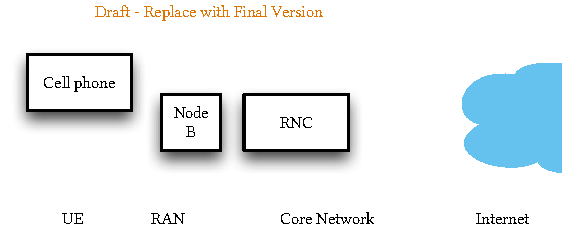
\includegraphics{cloud/virtualized_network_functions/measurement_data/figures/mobile_network_overview}
  \caption{Overview of the \headershortacr{METAWIN} monitoring architecture in a \headershortacr{3G} mobile network~\cite{Ricciato2006}.}
  \label{fig:cloud:virtualized_network_functions:measurement_data:dataset_description:mobile_network_overview}
\end{figure}

For this investigation we employ \gls{GTP} protocol data gathered by \gls{METAWIN}.
This data includes the \gls{RAT} identifier as well as the terminal types of the mobile clients, by use of the \gls{TAC} part of the \gls{IMEI}.
To meet privacy requirements, \gls{METAWIN} anonymises all captured data.
The application-level payload is removed and all user identifiers are hashed with one-way functions before data storage.
Individual \glspl{UE} in our dataset can be differentiated by the hashed \gls{MS-ID}, but not traced back to the actual user.

The used dataset is a week-long trace from the third week of April 2011.
It consists of \(2.2\) billion aggregated flows for user traffic and \(410\) million \gls{GTP} Tunnel Management transactions.
It was tapped at one of the \glspl{GGSN} of the operator and contains about half of the total traffic volume handled by the operator in this period.

\subsubsection*{Statistical Evaluation}\label{sec:cloud:virtualized_network_functions:measurement_data:evaluation}

Using this dataset, we can obtain the distributions required for the models introduced in \refsec{sec:cloud:virtualized_network_functions:model}.
First, we study the tunnel inter-arrival time in \reffig{fig:cloud:virtualized_network_functions:measurement_data:evaluation:tunnel_iat}.

\begin{figure}
  \centering
  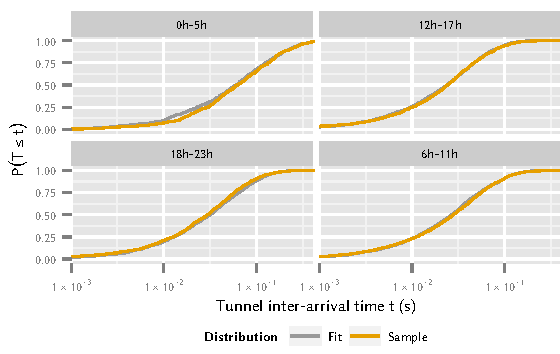
\includegraphics{cloud/virtualized_network_functions/measurement_data/figures/tunnel_iat}
  \caption{Empirical and exponentially fitted \headershortacrpl{CDF} of the tunnel inter-arrival duration by time of day. \headershortacrpl{CDF} are overlapping as the coefficient of determination is close to \(1\).}
  \label{fig:cloud:virtualized_network_functions:measurement_data:evaluation:tunnel_iat}
\end{figure}

The arrival of new tunnel requests can be used as a measure for the load a \gls{GGSN} experiences, as every incoming tunnel carries several signalling interactions, processing and state with it.
Typically, a device will only hold one tunnel at a time, but this tunnel can be initiated and shut down in rapid succession, causing the aforementioned issues in the radio network.
The arrivals also show a strong diurnal effect, closely resembling patterns present in the actual user traffic:
We observe a decline of arrivals, i.e. longer inter-arrivals, late in the night and during the early morning hours with a peak rate in the afternoon and early evening.
To represent this time-of-day dependence in the model, the measurement was split into the four time slots displayed in the figure.
Each slot was then fitted with an exponential distribution by way of moment matching.
This results in the cumulative negative exponential distribution function \(F(x) = 1- e^{-\lambda x}, x \geq 0\) with \(\lambda\) given in \reftab{tab:cloud:virtualized_network_functions:measurement_data:evaluation:iat_fits} for the four time slots.
The fitted functions match the empirical data, with some deviation present at the left tail but overall with a positive correlation coefficient approaching \(1\).

\begin{table}
  \centering
  \caption{Parameters for the exponentially distributed inter-arrival times and corresponding Pearson correlation coefficients.}
  \label{tab:cloud:virtualized_network_functions:measurement_data:evaluation:iat_fits}  
  \begin{tabular}{lcc}
  \toprule
  Time of day & \(\lambda\) & \(R_{arr}\)\\
  \midrule
  0h-5h & $10.67$ & $0.99$\\
  6h-11h & $24.53$ & $0.99$\\
  12h-17h & $29.25$ & $0.99$\\
  18h-23h & $23.49$ & $0.98$\\
   \bottomrule
  \end{tabular}
\end{table}

The second important tunnel property is the duration of the \gls{PDP} Context state accompanying a \gls{GTP} tunnel held at the \gls{GGSN}.
\reffig{fig:cloud:virtualized_network_functions:measurement_data:evaluation:tunnel_duration} shows the tunnel durations split up for the time of day, as there is once again a slight diurnal effect present, albeit with shifted peaks.
Longer tunnels tend to occur at night, shorter tunnels during midday.
Further properties of the tunnel duration, especially the correlation with device types and operating systems, are investigated in detail in~\cite{Metzger2014}.

\begin{figure}
  \centering
  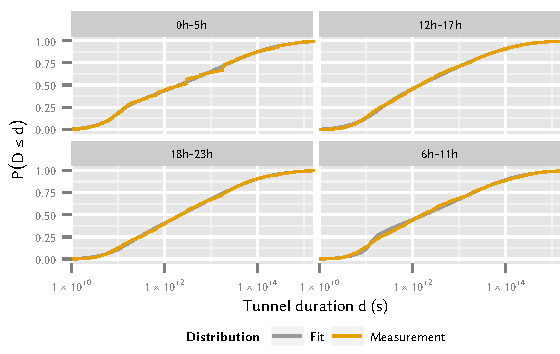
\includegraphics{cloud/virtualized_network_functions/measurement_data/figures/tunnel_duration}
  \caption{Empirical and fitted \headershortacrpl{CDF} of the tunnel duration by time of day with fitted rational functions.}
  \label{fig:cloud:virtualized_network_functions:measurement_data:evaluation:tunnel_duration}
\end{figure}

\begin{table}
  \centering
  \caption{Inverse functions fitted to the empirical duration distribution and correlation coefficients of the fit.}
  \label{tab:cloud:virtualized_network_functions:measurement_data:evaluation:duration_fits}  
  \begin{tabular}{lcc}
  \toprule
  Time of day & Inverse fitted duration function & \(R_{dur}\)\\
  \midrule
  0h-5h & $0.91 - 60.61y - 3498.78y^3 - \frac{110.70y + 2289.94y^3}{y - 1.00}$ &  $0.99$ \\
  6h-11h & $1 + 117.48y - 368.64y^2 - \frac{1720.13y^4}{y - 1.00}$ & $0.99$ \\
  12h-17h & $0.95 + 69.49y + \frac{81146.10y^3 + 1.08\times10^6y^5}{805 - 802.01y}$ & $0.99$ \\
  18h-23h & $0.91 + 82.05y - \frac{2936.93y^4}{1.94y - 1.95}$ & $0.99$\\
  \bottomrule
  \end{tabular}
\end{table}

Furthermore, the model requires information on the tunnel durations.
However, none of the basic probability distributions, e.g. exponential, gamma, and Weibull distributions, fit the tunnel duration well enough.
One of the reasons for this probably being the correlation of the tunnel duration to a large number of factors, including user behaviour and network-specific timers and procedures, e.g. tunnels are shut down by the network after specific events, introducing artefacts which make it hard to fit any distribution against.
Instead, we fit rational functions to the empirical \gls{CDF} using the Eureqa \cite{Schmidt2009} software.

This allows for a much closer fit while still smoothing out some of the artefacts.
\reftab{tab:cloud:virtualized_network_functions:measurement_data:evaluation:duration_fits} displays these functions fitted to the inverse \gls{CDF}, to be directly used for generating random numbers using the inversion method.
Both the \gls{CDF} in \reffig{fig:cloud:virtualized_network_functions:measurement_data:evaluation:tunnel_duration} as well as the Pearson correlation coefficient confirm the goodness of the fitted functions.

\subsection{Comparison of Traditional and Virtualised Approach}\label{sec:cloud:virtualized_network_functions:performance_evaluation}

We implement the models introduced in \refsec{sec:cloud:virtualized_network_functions:model} using a \gls{DES} with the SimPy\footnote{\url{https://simpy.readthedocs.org/}, \accessed} package as foundation.
The implementation\footnote{\url{https://github.com/fmetzger/ggsn-simulation/}, \accessed} as well as the considered scenarios\footnote{\url{https://github.com/cschwartz/ggsn-simulation-studies/}, \accessed} are also publicly available as a reference.
To be in line with the measurement data we consider a simulation time for all simulation scenarios of 7 days, with a transient phase of 60 minutes.
Ten replications of each scenario were performed.
All error bars given in this section show the \SIrange{5}{95}{\percent} quantiles of all replications.

We use the measurements introduced in \refsec{sec:cloud:virtualized_network_functions:measurement_data} in order to dimension a traditional \gls{GGSN} as a baseline for all further studies.
Based on these results, we first examine the effects of network function virtualisation by scaling \emph{out} instead of up through a virtual \gls{GGSN} model.
Finally, we arrive at a more realistic version of the virtual \gls{GGSN} by taking the start-up and shut-down times into account.

\subsubsection*{Traditional \headershortacr{GGSN}}\label{sec:cloud:virtualized_network_functions:performance_evaluation:traditional_ggsn}

Employing the inter-arrival times and duration of tunnels, we first study the traditional \gls{GGSN} model introduced previously.
Whilst our measurements provide us with information on the frequency of new tunnels and the duration they remain active, we have no reliable information on the number of active tunnels the \gls{GGSN} can support.
Thus, in a first step, we dimension the \gls{GGSN} in such a way that a suitable blocking probability \(\blockingprobability\) can be achieved.

In order to obtain a baseline dimensioning, we perform a simulation study, considering the impact of an increasing offered load on the blocking probability.
We observe that as the number of supported parallel tunnels increases, the blocking probability decreases.
For the normalized inter-arrival no blocking is occurring if we allow for more than \(5000\) parallel tunnels.
Thus, we consider the range of \(4000\) to \(5000\) parallel tunnels to be of special interest for the remainder of the study.

\subsubsection*{Virtual \headershortacr{GGSN}}\label{sec:cloud:virtualized_network_functions:performance_evaluation:virtual_ggsn}

To study the feasibility of the virtual \gls{GGSN} approach discussed in \refsec{sec:cloud:virtualized_network_functions:model}, we compare the performance metrics of the virtual \gls{GGSN} with that of a traditional \gls{GGSN}.
To this end, the virtual \gls{GGSN} is simulated in varying configurations.
The number of servers and supported tunnels per server is chosen in such a way that the results can be compared with those obtained from our study of the traditional \gls{GGSN}.
Due to simulation time constraints, only a representative subset of scenarios is simulated.

In the virtual \gls{GGSN} model, servers are activated and deactivated on demand, while in the traditional \gls{GGSN} model, the single server is always on.
For this investigation a conservative start-up and shut-down time \(d\) of \SI{300}{\second} is chosen.
Generally, deactivating server instances reduces energy consumption, frees up inactive servers for other use, or reduces cost to be paid to a cloud operator.
For this reason, the number of active servers \(I\) is a relevant performance metric in the virtual \gls{GGSN} model.

\begin{table}\caption{Manipulation check for the experimental factors based on one-way ANOVA.}
\centering
\label{tab:cloud:virtualized_network_functions:performance_evaluation:virtual_ggsn:manipulation}
\tabcolsep=0.11cm
\begin{tabular}{lccccc}
\toprule
& \(F(2,1275)\) & \(\eta^2_p\) & \(p\) & Cohen's & Cohen's\\
&  & & & \(f^2\) & \(\hat{\omega}^2\) \\
\midrule
\emph{blocking probability} \(\blockingprobability\)  & & & & &\\
maxTunnels \(n\)&  15601.53 & \textcolor{red}{0.993} & $<0.001$ & \textcolor{red}{26.73} & 0.96\\
maxInstances \(\maxServers\)&  10218.17 & \textcolor{red}{0.986} & $<0.001$ & \textcolor{red}{1.06} & 0.51\\
startstopDuration \(d\) &  0.86 & \textcolor{black}{0.003} & $0.482$ & \textcolor{black}{0.00} & 0.00\\
\midrule
\emph{mean tunnel count} \(n_A\) & & & & &\\
maxTunnels \(n\)&  20448.34 & \textcolor{red}{0.994} & $<0.001$ & \textcolor{red}{27.71} & 0.96\\
maxInstances \(\maxServers\)&  13348.25 & \textcolor{red}{0.989} & $<0.001$ & \textcolor{red}{1.06} & 0.51\\
startstopDuration \(d\) &  2.87 & \textcolor{black}{0.009} & $0.022$ & \textcolor{black}{0.00} & 0.00\\
\bottomrule
\end{tabular}
\end{table}

For the analysis of the influence of different model parameters on the performance metrics, we perform a one-way ANOVA with the results in \reftab{tab:cloud:virtualized_network_functions:performance_evaluation:virtual_ggsn:manipulation}.
High values for the effect size estimators \(\eta_p^2\) and Cohen's \(f^2\)\cite{Ellis2010} indicate that the main influence for both blocking probability \(\blockingprobability\) and mean number of tunnels \(n_A\) is the maximum number of tunnels \(n\) and virtual \gls{GGSN} instances \(\maxServers\), i.e. the total number of possible concurrent tunnels in the system.
Therefore, we study these parameters first.

\begin{figure}
  \centering
  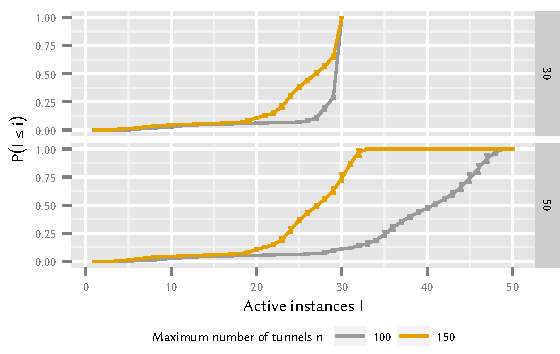
\includegraphics{cloud/virtualized_network_functions/performance_evaluation/figures/instanceuse_multiserver}
  \caption{Impact of the maximum number of tunnels \(n\) and number of servers \maxServers on number of active servers in the virtual \headershortacr{GGSN} model.}
  \label{fig:cloud:virtualized_network_functions:performance_evaluation:virtual_ggsn:instanceuse_multiserver}
\end{figure}

In \reffig{fig:cloud:virtualized_network_functions:performance_evaluation:virtual_ggsn:instanceuse_multiserver} the \gls{CDF} of the number of active servers for four different virtual \gls{GGSN} configurations is displayed.
We study the behaviour of a virtual \gls{GGSN} with \(\maxServers = 30\) servers, where each server can support \(n = 100\) or \(n = 150\) tunnels.
Then, we compare this with a virtual \gls{GGSN} with \(\maxServers = 50\) servers and again \(n = 75\) or \(n = 150\) tunnels.
We observe that increasing the number of supported tunnels \(n\) per server allows a larger percentage of servers to be shut-down or used for other tasks. This demonstrates the scaling capability of the virtualised model quite well.
Note that both the scenario with \(30\) servers \maxServers and \(150\) maximum tunnels \(n\) per server as well as the scenario with \(60\) servers \maxServers and \(75\) maximum tunnels per server sharing the same maximum amount of tunnels, i.e. \(4500\), being right at the centre of the interesting range of candidates.

\begin{figure}
  \centering
  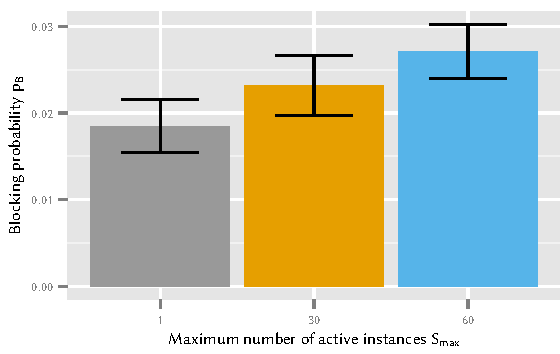
\includegraphics{cloud/virtualized_network_functions/performance_evaluation/figures/blocking_comparison}
  \caption{Impact of blocking probability \blockingprobability on the number of servers compared to the traditional \headershortacr{GGSN}, \(4500\) maximum tunnels per server being on a single server, i.e. \(150\) on \(30\), and \(75\) on \(60\) servers.}
  \label{fig:cloud:virtualized_network_functions:performance_evaluation:virtual_ggsn:blocking_comparison}
\end{figure}

Next, we study the blocking probability of the virtual \gls{GGSN} system in \reffig{fig:cloud:virtualized_network_functions:performance_evaluation:virtual_ggsn:blocking_comparison} and compare it to the results from the traditional \gls{GGSN} model with both systems dimensioned for \(4500\) tunnels.
We observe that, considering the start-up and shut-down time of \SI{300}{\second}, the blocking probability \blockingprobability increases by a factor of \(1.46\) if the virtual \gls{GGSN} is comprised of \(60\) instances \(\maxServers\) dimensioned for \(75\) concurrent tunnels \(n\) , i.e. \(\frac{1}{60}\) of the original server capacity.
In this case \(27\) of all \(60\) servers can be turned off or used for other purposes at \SI{50}{\percent} of the time.
We conclude that choosing more powerful servers decreases the blocking probability but reduces the potential to disable servers.

So far we have considered a conservative start-up and shut-down time of servers \(d\) of 5 minutes, which can potentially occur in non-virtualised available hardware.
In the next section we study the impact of reduced start-up and shut-down times with modern servers with fast storage, e.g. \glspl{SSD}, or containerised applications\footnote{\url{https://www.docker.com/}, \accessed}.

\subsubsection*{Impact of Start-up and Shut-down Times}\label{sec:cloud_virtualized_network_functions:startup_shutdown}

In this section, we first consider the impact of different start-up and shut-down times \(d\) on resource utilisation \(n_A\) and blocking probabilities \blockingprobability.
Afterwards, the influence of varying server start and stop times \(d\) on a fixed combination of maximum tunnels \(n\) and servers \maxServers in the system is examined.

\begin{figure}
  \centering
  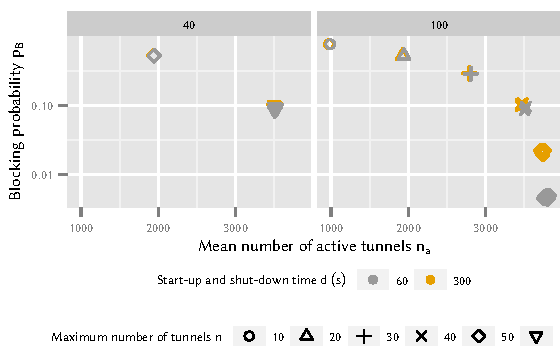
\includegraphics{cloud/virtualized_network_functions/performance_evaluation/figures/compare_util_block}
  \caption{Trade-off between blocking probability \blockingprobability and mean resource utilisation \(n_A\) with regard to maximum number of instances \maxServers, maximum number of tunnels per server \(n\), and start-up and shut-down time \(d\).}
  \label{fig:cloud_virtualized_network_functions:startup_shutdown:compare_util_block}
\end{figure}

\reffig{fig:cloud_virtualized_network_functions:startup_shutdown:compare_util_block} shows scenarios with \(40\) and \(100\) \gls{GGSN} instances \(maxServers\) and  \(1000\) to \(5000\) total concurrent tunnels.
For each scenario, we study the impact of selecting a different maximum number of tunnels \(n\) per server as well as start-up and shut-down times \(d\) on blocking probability \blockingprobability and mean resource utilisation \(n_A\).
The first observation is that by increasing the number of servers \(\maxServers\), i.e. scaling out, the blocking probability \blockingprobability can be decreased, while maintaining a relatively low mean resource utilisation \(n_A\).
In addition to the previous effects, we notice that a higher start-up and shut-down time \(d\) causes a slight increase in blocking probability \blockingprobability for servers with low tunnel capacity \(n\).

\begin{figure}
  \centering
  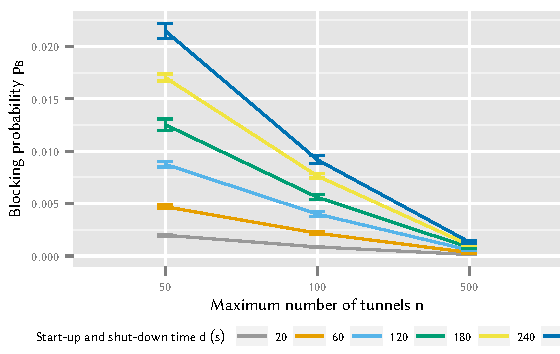
\includegraphics{cloud/virtualized_network_functions/performance_evaluation/figures/compare_maxinstances_block}
  \caption{Influence of start-up and shut-down time \(d\) on blocking probability \(p_B\) with regard to different numbers of supported tunnels per instance \(n\).}
  \label{fig:cloud_virtualized_network_functions:startup_shutdown:compare_maxinstances_block}
\end{figure}

We focus on a specific scenario in \reffig{fig:cloud_virtualized_network_functions:startup_shutdown:compare_maxinstances_block}, where \(5000\) total tunnels should be supported by the system, to study this behaviour in more detail.
To achieve this goal, we consider three types of instances, with the server capacity \(n\) varying between \(50\) and \(500\).
In each case we change the start-up and shut-down time \(d\) between \(20\) and \(\SI{300}{\second}\).
We observe that lower server capacities \(n\) combined with higher start-up and shut-down times \(d\) increase the blocking probability \blockingprobability.
This is due to the server start-up threshold mechanism, used in the model, not taking the additional capacity gained by activating an additional server into account.
If a low capacity server with a long boot time is activated, there is a high probability that the system will quickly expend its capacity again.

Thus, it can be concluded that if smaller instances are to be used, e.g. due to the fact that they are cheaper than large instances, start-up and shut-down times should be kept minimal, for example by using containers or \glspl{SSD}.
